\documentclass[12pt]{scrartcl}

\usepackage{amsthm}
\usepackage{ocgx}
\usepackage{amsmath}
\usepackage{svg}
\usepackage{graphicx}
\usepackage{pgfplots}


\title{Lecture Notes week 1}
\author{\"Omer \c Sakar}
\date{15 November 2016}

\newtheorem{defi}{Definition}
\newtheorem{theo}{Theorem}

\pgfplotsset{width=10cm,compat=1.9}
%\usepgfplotslibrary{external}
%\tikzexternalize

\begin{document}
\maketitle
\tableofcontents
\newpage

\section{Lecture 1}
There were no notes made during lecture one, because I had no idea that it was a lecture.


\newpage
\section{Lecture 2 Strenght of weak ties \\ \ \ \ Chapter 3 and 4} 

\subsection{Triadic closure}
\begin{defi}
	$\#wedges(A) = \binom{d(A)}{2} = \frac{d(A)*(d(A)-1)}{2} $
\end{defi}

\begin{defi}
	$Clustering\ coefficients\ c(A) = \frac{\#\ \Delta\ with\ A}{\#\ wedges\ through\ A}$
\end{defi}

\noindent Examples from the slides: \newline
The triangles with A are: $CAO,\ OAF,\ CAB,\ CAD,\ DAB,\ BAF,\ FAG\ and\ BAG\ $ (8 in total) and the triangle with H is: $LHM$ (1 in total).

\noindent $d(A) = 6 \Rightarrow c(A) = \frac{8}{6\cdot 5/2} = \frac{8}{15}$ \newline 
$d(H) = 4 \Rightarrow c(A) = \frac{1}{4\cdot 3/2} = \frac{1}{6}$ \newline


\subsection{Bridges}
\begin{defi}
	Bridge: An edge between u and v is a bridge if deleting this edge results in u and v lying in different components.
\end{defi}
\begin{defi}
	Local bridge: Edge uv is a local bridge if deleting this edge results in a path $>$ 2 between u and v.
\end{defi}

\noindent Question: Let $uv$ be a local bridge. How many friends do $u$ and $v$ have in common?
\switchocg{refmyfirstocg}%
{\textcolor{red}{Click here to show answer}}

\begin{ocg}{My first OCG}{refmyfirstocg}{1}
\noindent Answer: None. If $u$ and $v$ have a friend in common, the path from $u$ and $v$ would be 2 ($u \rightarrow friend  \rightarrow v$). Thus it is not be a bridge anymore. 
\end{ocg}

\subsection{Strong and weak ties}
\begin{defi}
	$A$ violates the strong triadic closure property ($STC$), if it has strong ties to 2 other nodes $b$ and $c$ and there exists no (strong or weak) tie between $b$ and $c$.
\end{defi}

\noindent See slides for and exercise on strong and weak ties.

\begin{theo}
	If A satisfies the STC and has $\geq$ 2 strong ties, then any local bridge incolving A is a weak tie.
\end{theo}

\noindent Example in the slides:
Question: $FI$ is a local bridge. Proof that $FI$ is weak. \newline

Informal answer: If $FI$ was strong, the edge $GI$ would exist. If the edge $GI$ existed, $FI$ would not be a local bridge anymore. Thus a contradiction $\bot$.

\begin{minipage}{0.5\textwidth}
	Formal answer: $\exists$ c such that the edge $AC$ is a strong tie ($A$ has at least one more string tie). The STC implies that $CB$ must now be a tie. This means $AB$ is not a local bridge, because the path $(A \rightarrow C \rightarrow B)$ is of length two.
\end{minipage} \hfill
\begin{minipage}{0.3\textwidth}	
	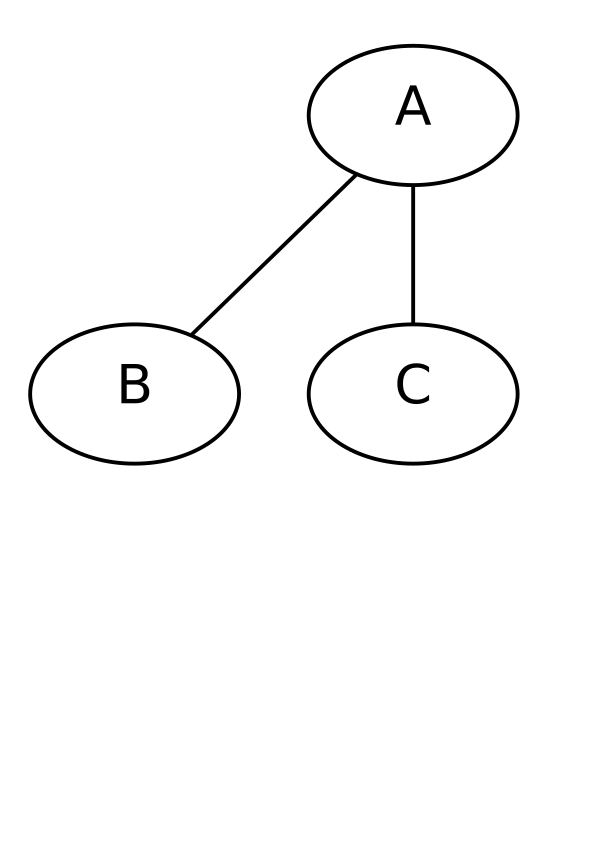
\includegraphics[width=0.69\textwidth]{./images/formal_proof_ties.pdf}
    \label{fig:formal_proof_ties}
\end{minipage}


\subsection{Embeddedness of an edge}
\begin{defi}
	Embeddedness of an edge AB = \# common neighbours of A and B
\end{defi}

\begin{defi}
	Neighbourhood overlap of AB = $\frac{Embeddednes\ of\ AB}{\#\ nodes\ that\ are\ neighbours\ of\ A\ or\ B}$
\end{defi}
\noindent Examples on the slides:\newline
Neighbourhood overlap AB = $\frac{4}{6}$ = $\frac{2}{3}$\newline
Neighbourhood overlap FI = $\frac{0}{6}$ = $0$ (FI is a local bridge)\newline
Neighbourhood overlap FG = $\frac{2}{5}$\newline

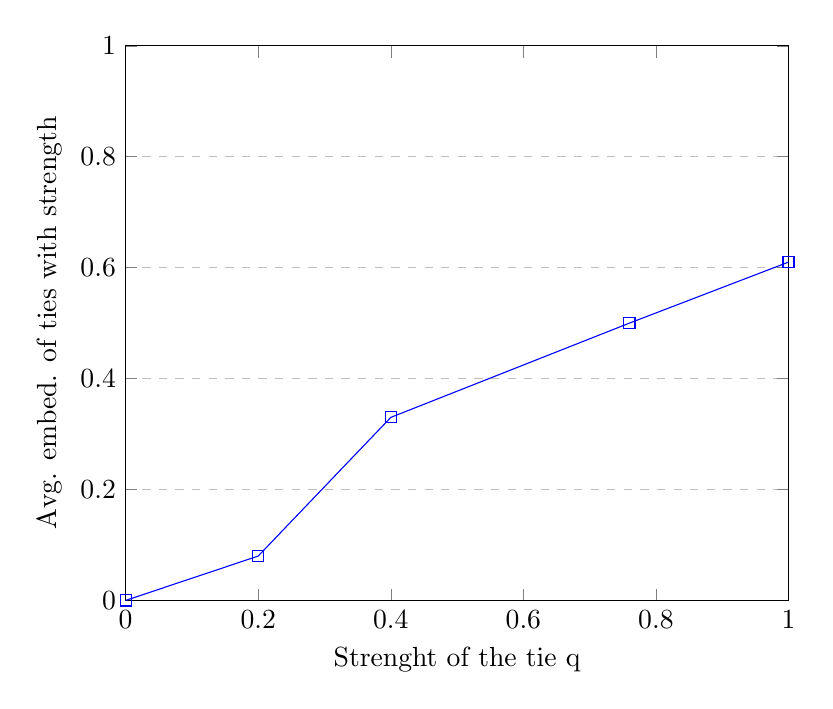
\begin{tikzpicture}
\begin{axis}[
    xlabel={Strenght of the tie q},
    ylabel={Avg. embed. of ties with strength},
    xmin=0, xmax=1,
    ymin=0, ymax=1,
    xtick={0,0.2,0.4,0.6,0.8,1},
    ytick={0,0.2,0.4,0.6,0.8,1},
    legend pos=north west,
    ymajorgrids=true,
    grid style=dashed,
]
 
\addplot[
    color=blue,
    mark=square,
    ]
    coordinates {
    (0,0)(0.2, 0.08)(0.4,0.33)(0.76,0.5)(1,0.61)
    }; 
\end{axis}
\end{tikzpicture}

$q = fraction of edges with strengh \leq w$

\subsection{Linked prediction using number of common friends}
Base\_line: each common friend given probability p to meet, independent of other common friends.\newline

\noindent$P(meet on given day | k common friends) = 1 - (1-p)^k$ \newline
Since p is small: $1 - (1-p)^k = \sum_{i=0}^{k} \binom{k}{i} \cdot (-1)^k \cdot p^k = 1 - kp + O(p^2) = 1 - kp$

\begin{minipage}{0.3\textwidth}	
	\includegraphics[scale=0.4]{./images/figure49.pdf}
\end{minipage}

\subsection{Homophily}
Due to incomprehensible notes, this section is ommited. Voor zover ik het herinner was dit stuk ook niet verplicht. Ze had haat aan dit stukje van het boek en dat wou ze uiten.



\end{document}




